\chapter{Implementation}
\label{implementation}

The implementation section outlines the features that have been implemented from the designs outlined in the previous chapter. It also covers the technical details of how particular components of the system operates including algorithm breakdowns and results from preliminary testing where necessary. \\

\section{System Implementation}

The implementation of the system describes each component as it was implemented in the final system. In this section, the broad functionality of each component is described. Further subsections discuss the overall accuracy and results achieved from the components implemented. \\

\subsection{CoreLoader}

The main Coreloader screen contains all functionality associated with the system. There are options present for selecting particular Kinect feeds, calibrating the Kinect's position and viewing the debug console. Recent patients are also displayed persistently for quick access to the scans and results of previous scans on a particular patient. Configuration options are also possible through Coreloader such as setting the working directory for PARSE files and attributing .PARSE and .PCD scan files to patients. Exporting scans to .PCD is also here so that scans produced by the System can be visualised using the Point Cloud Library toolkit\footnote{Point Cloud Library, http://www.pointclouds.org}. \\

\begin{center}
    
\includegraphics[scale=0.5]{zscreenshots/corewelcome.png}\\
    \caption{CoreLoader welcome screen with toolkit options}
\end{center} \\

\begin{center}
    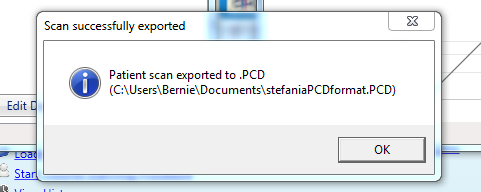
\includegraphics[scale=0.6]{zscreenshots/savetopcd.PNG}\\
    \caption{Confirmation of point cloud file exported to .PCD}
\end{center} \\

\begin{center}
    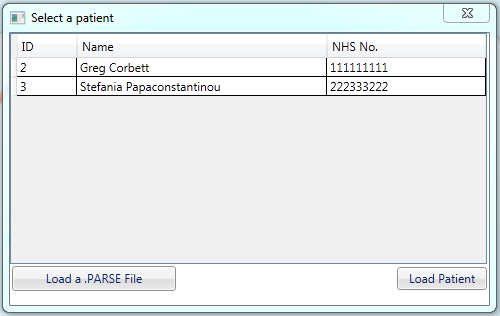
\includegraphics[scale=0.55]{zscreenshots/metaloader.PNG}\\
    \caption{List of patients in the database with associated point cloud or scan information}
\end{center} \\

\begin{center}
    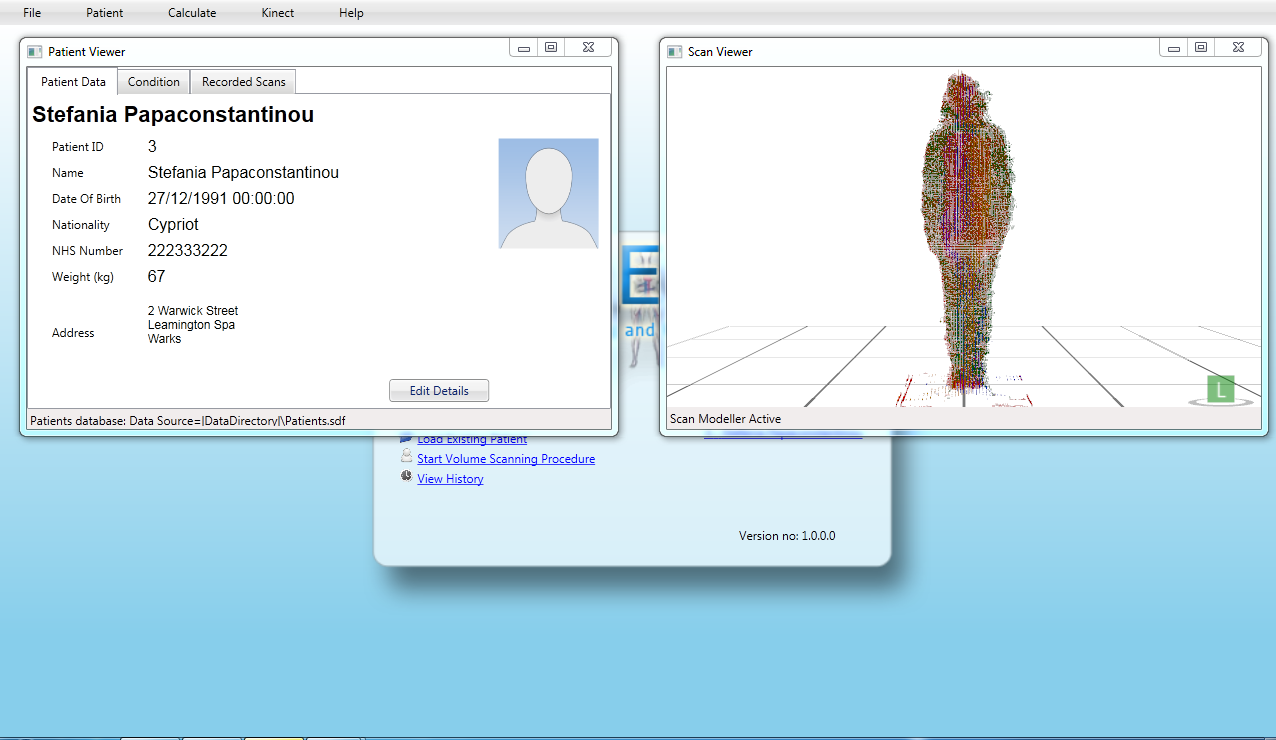
\includegraphics[scale=0.3]{zscreenshots/coreloaderstef.PNG}\\
    \caption{System with scan and associated patient detail displayed}
\end{center} \\


\subsection{ViewLoader}

\begin{center}
    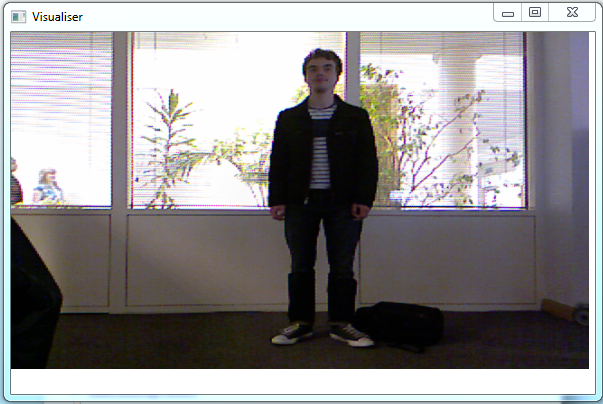
\includegraphics[scale=0.5]{zscreenshots/rgbvisualiser.PNG} \\
    \caption{ViewLoader: Showing the raw RGB feed}
\end{center} \\

Viewloader is capable of displaying raw streams from the Kinect or composite streams that combine multiple views such as depth isolation, colour isolation, or the overlay of a skeleton onto existing feeds. The above image shows the conventional RGB feed from the Kinect. \\

\subsection{ScanLoader}

\begin{center}
    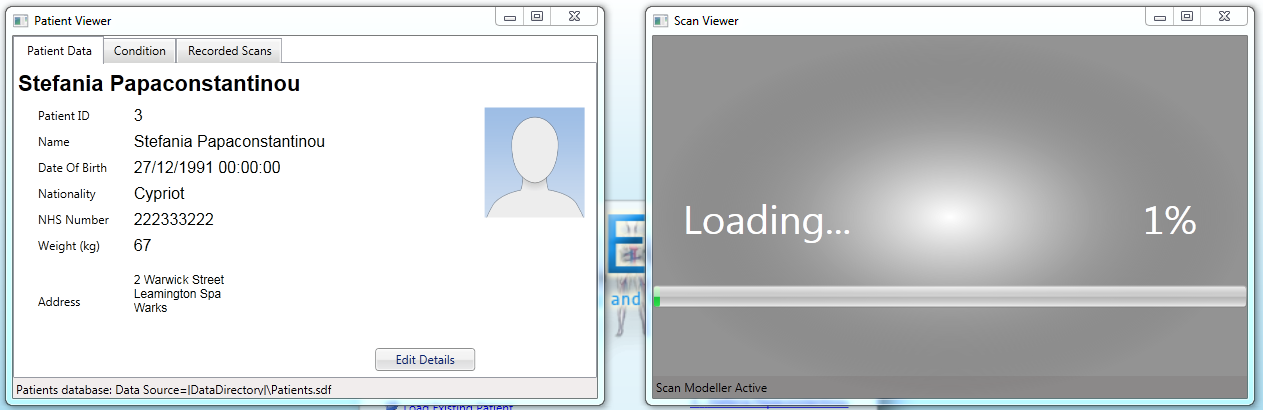
\includegraphics[scale=0.3]{zscreenshots/patientloading.png} \\
    \caption{ScanLoader: The patient data portal (left) and the model viewer loading (right)}
\end{center} \\

\begin{center}
    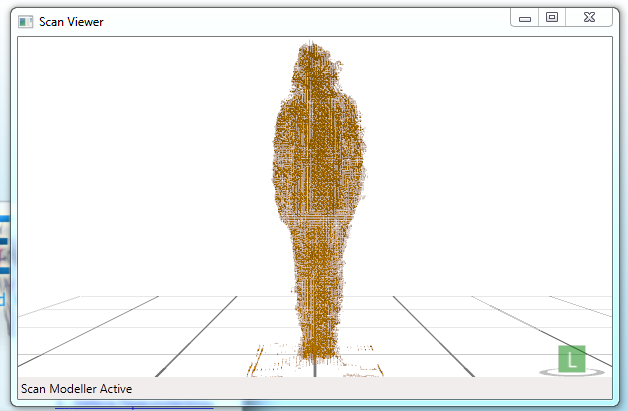
\includegraphics[scale=0.5]{zscreenshots/scanframework.png} \\
    \caption{ScanLoader: 3D model viewport}
\end{center} \\

ScanLoader visualises the registered point clouds from the scan process and allows the model to be viewed from a number of different perspectives and zoom levels. The point cloud visualisation process is resource intensive as approximately 200,000 points are drawn in 3D space. As a result of this, a persistent loading dialog is displayed when the point cloud is being loaded into scan loader or when refining operations are applied to the point cloud. \\

\subsection{HistoryLoader}

\begin{center}
    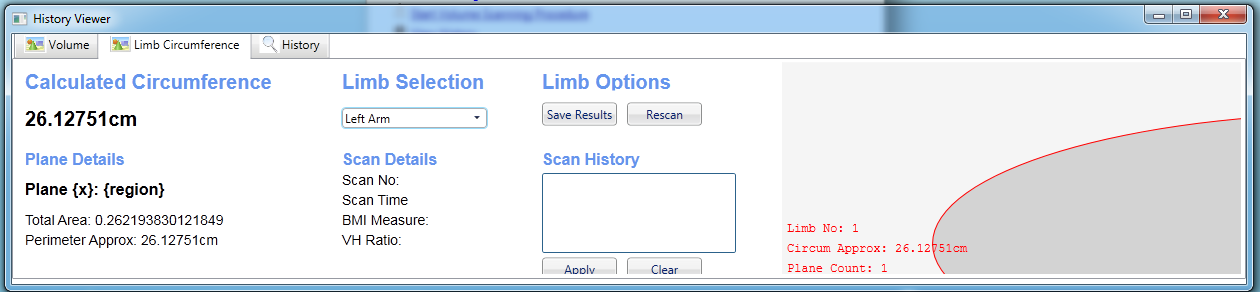
\includegraphics[scale=0.4]{zscreenshots/circumdetail.png}
    \caption{HistoryLoader: Circumference history}
\end{center} \\

\begin{center}
    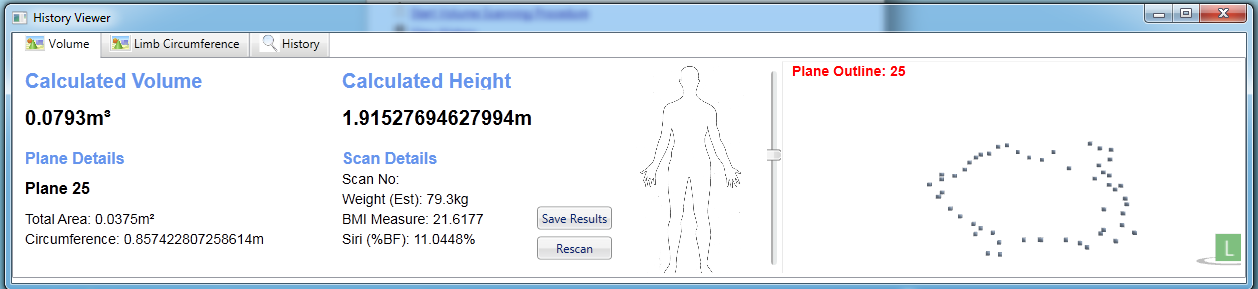
\includegraphics[scale=0.4]{zscreenshots/voldetail.png}
    \caption{HistoryLoader: Volume, height \& plane history}
\end{center} \\

\begin{center}
    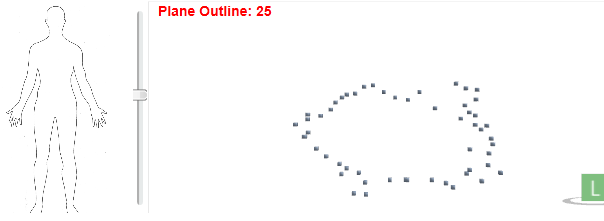
\includegraphics[scale=0.75]{zscreenshots/volumevisualisation.png}
    \caption{HistoryLoader: Plane viewer}
\end{center} \\

The HistoryLoader component of the system visualises the volume and circumference calculation results along with visualisations related to the extrcted planes from the point cloud as well as the visualisation for the approximation of the circumference of the limbs. In each component, different metrics can be visualised for volume in terms of the different planes of the body as well as the circumference for each limb that has been partitioned. These results can then be saved or refined during a rescan procedure. \\

\subsection{PatientLoader}

\begin{center}
    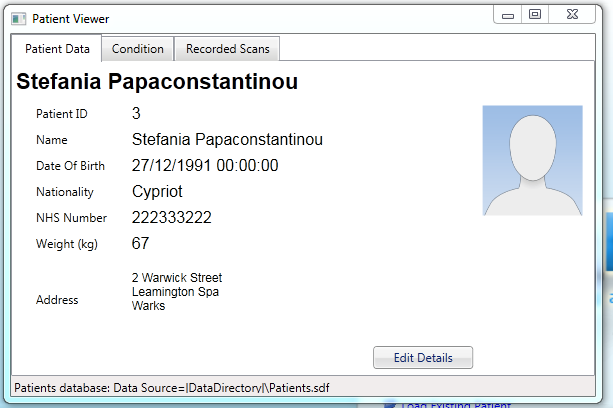
\includegraphics[scale=0.5]{zscreenshots/patientdetail.png} \\
    \caption{PatientLoader: Patient information pane}
\end{center} \\

The PatientLoader presents the patient detail recovered from the database when a patient's scans for either volume/limb circumference or markerless recognition purposes is loaded. PatientLoader also provides the ability to apply new markerless measurements and recover old measurements. Patient information such as personal details and patient conditions can also be added here. \\

\subsection{MeasurementLoader}
MeasurementLoader presents the mechanism for adding a new body-relative scan position with a hand-held sensor. Clear instructions are displayed, indicating to the users how to progress.\\

\begin{enumerate}
    \item Wait for two people to be in view
    \item Search for the sensor device
    \item Use the sensor's location, in combination with the skeletal data, to identify the doctor and the patient
    \item When the sensor is held still for 10 seconds, the system automatically runs the capture routine.
\end{enumerate} \\

\begin{center}
    \setlength\fboxsep{0pt}
    \setlength\fboxrule{0.5pt}
    \fbox{
\includegraphics[scale=0.25]{zscreenshots/MeasurementLoader.png}}\\
    \caption{MeasurementLoader: Ready to start a scan}
\end{center} \\

\begin{center}
    \setlength\fboxsep{0pt}
    \setlength\fboxrule{0.5pt}
    \fbox{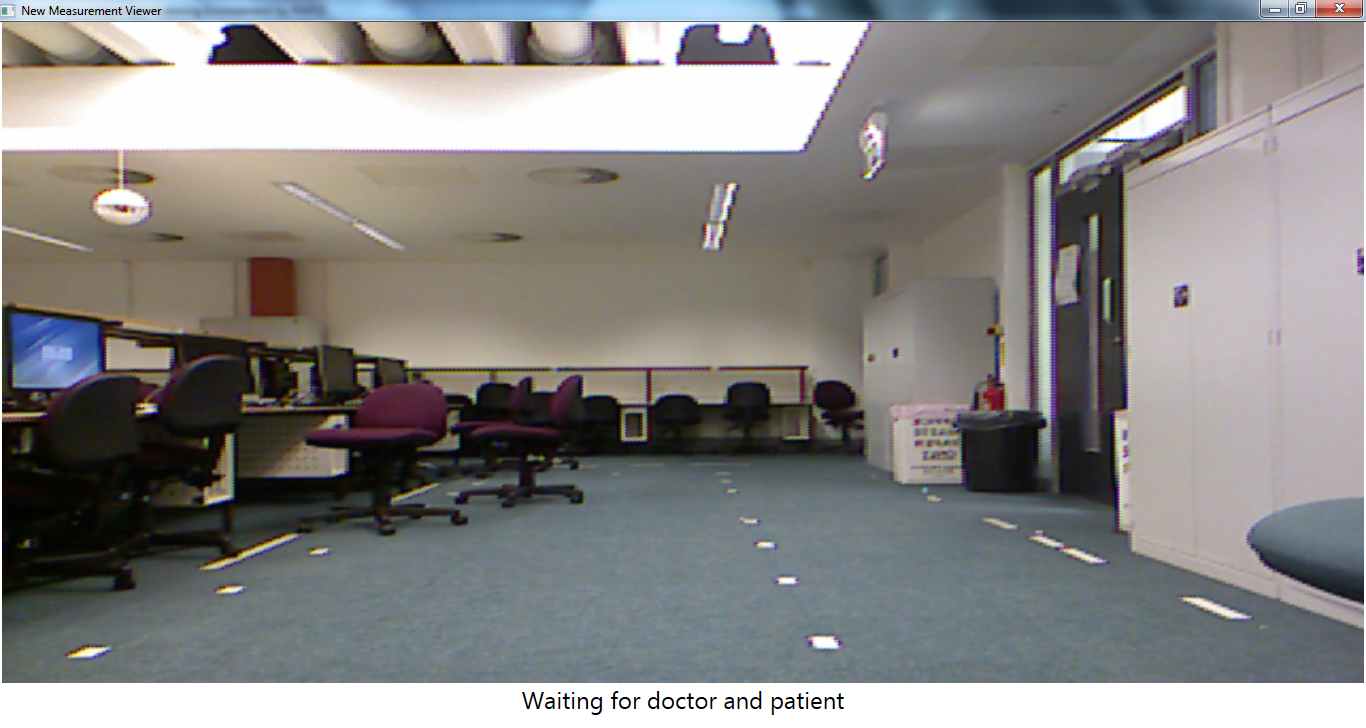
\includegraphics[scale=0.25]{zscreenshots/MeasurementLoader2.png}}\\
    \caption{MeasurementLoader: The large, clear display indicates the next step}
\end{center}


%\section{External Libraries}
A number of external libraries have been used to provide data abstraction and optimised functionality. This section will explore details about their licensing and usage within the PARSE toolkit. \\

\subsection{Kinect SDK}
The Kinect SDK was the basis for the development of the project but the group only utilised a subset of it's functionality as our specialist point cloud reconstruction and volume estimation required access to the raw depth feed as necessitated for reconstructing the body. The SDK itself provided a means of accessing functions which allowed data to be mapped onto different coordinate spaces for the reconstruction of the point cloud. The Skeletal tracking technology also provided by the Kinect was used extensively in order to when a body is in view of the kinect for calibration, scanning, and markerless recognition purposes. It has also been used for the basis of isolation as it provided useful cues as to the appropriate level at which to perform a depth cut off. \\ 

\subsection{Math.NET}
A library called Math.NET was utilised extensively in the ICP portion of the solution to make up for the lack of support for data structures representing matrices and their associated operations within C# and the .NET framework \cite{mathdotnet}. The framework only contained basic operations such as additive and multiplicative operations and contained only a small subset of the operations that are available in an application such as MatLAB. Due to the lack of free matrix manipulation libraries Math.NET was used as a compromise and much of the matrix manipulation functionality was re-implemented in a specialised manner for this project. It is available under the MIT/X11 license which is a permissive licence allowing the usage of the software in both free and commercial applications as long as attribution is given \footnote{Fulltext available at: http://www.xfree86.org/3.3.6/COPYRIGHT2.html}. \\

\subsection{Helix3D}
Helix3D is a WPF based visualisation framework which adds a number of helper functions and viewport interactivity to the existing WPF3D framework \footnote{HelixLink}. Since it's inception, WPF3D has generally been considered a poor alternative to more established high performance frameworks such as OpenGL \cite{WpfPoor} but due to our language choice and the declining support of DirectX, WPF3D combined with Helix provided an adequate means of visualising the reconstructed point clouds and planes extracted from segmented point clouds after volume calculation and limb circumference determination. \\  

\subsection{WpfToolkit}
\label{design:wpf}

WpfToolkit added further functionality to the Windows Presentation Framework such as charting and visualisation for Markerless recognition/recall tasks. \\
%\subsection{Database}
For the storage requirements of the toolkit, a database has been put in place and it is used to store the details of the patients and their scans and measurements. To assist in the storage and retrieval of information from the database a specific class has been designed, that includes all the required queries. All accesses to the database are done in a clean and efficient way by using parameterised queries (otherwise called prepared statements). This not only enables re-usability of queries for different tables and sets of data but also makes the usage of the database safer as they provide protection against SQL injection attacks. \\

\section{Person Isolation}
This section details the implementation of the person isolation methods described in Section \ref{design:person isolation}.\\

\subsection{Colour Based Isolation}
\label{imp:colour based isolation}
Figure \ref{fig:colour based cut off} shows the colour based isolation, described in Section \ref{design:colour based isolation}. As originally suspected, when implemented this method appears to perform well, removing all non-person details from the scene.\\

\begin{figure}[h]
    \begin{center}
        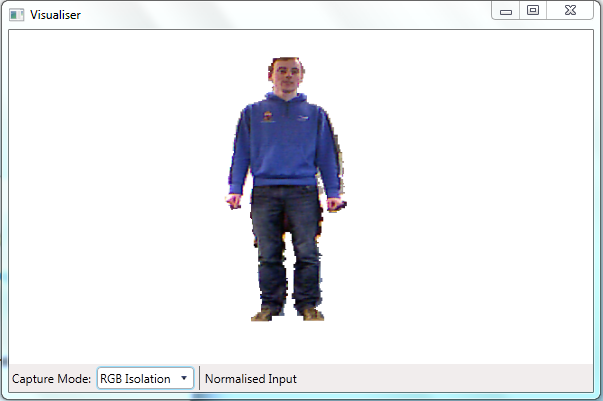
\includegraphics[scale=0.4]{images/parse4} 
    \end{center}
    \caption{Colour based isolation.}
    \label{fig:colour based cut off}
\end{figure} 

However, colour based isolation is not immediately useful as depth data is need to create the point cloud.\\ 

An attempt to overcome this was to try to map the colour pixels, which corresponded to a person, to depth pixels. Unfortunately, as the depth sensor and colour camera are not situated in the same place on the Kinect, see Figure \ref{fig:kinectoffset}, this mapping is non trivial and is currently an open problem in and of itself in the Kinect development community. Efforts were devoted by the group to fix or at least account for this problem, however none of the solutions proposed lead to a sufficiently isolated person. In Figure \ref{fig:a poorly isolated person}, it can be seen that colour based isolation leads to a poorly isolated person in depth space. The lack of effective mapping between colour and depth pixels also negated the possibility of a textured point cloud being displayed by the toolkit.\\

\begin{figure}[h]
\begin{center}
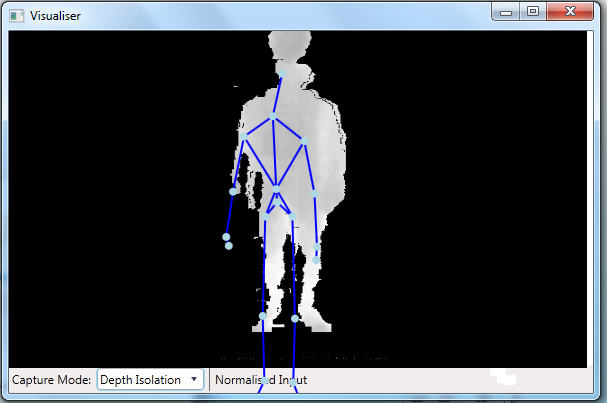
\includegraphics[scale=0.4]{images/parse5} 
\end{center}
\caption{A poorly isolated person.}
\label{fig:a poorly isolated person}
\end{figure} 

\subsection{Depth Based Isolation}
\label{imp:depth based isolation}
Figure \ref{fig:depth based cut off} shows the depth based isolation, described in Section \ref{design:depth based isolation}. As predicted, this cut appears to be sufficient to eliminate a large proportion of non-person data but does not remove the ring of points at the same depth as the person.\\

\begin{figure}[h]
\begin{center}
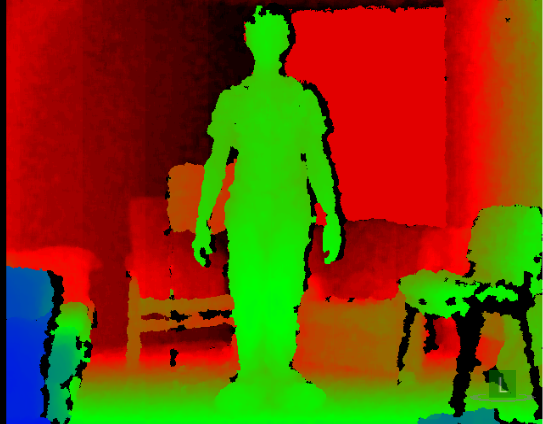
\includegraphics[scale=0.4]{images/parse1} 
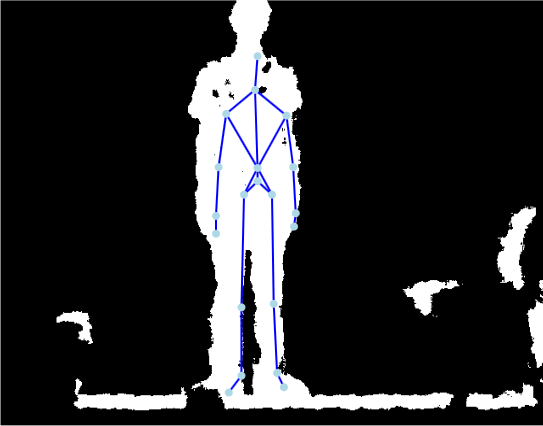
\includegraphics[scale=0.4]{images/parse2}
\end{center}
\caption{Depth based cut off, before (left) and after (right).}
\label{fig:depth based cut off}
\end{figure} 

Figure \ref{fig:depth and hand based cut off} hand based extension to the depth cut off. As predicted, the combination of using depth and hand position appears sufficient to isolate a person, although the floor beneath them does remain. As such, this method was chosen to isolate the person. To aid the creation of a point cloud, the isolated person is coloured from black to white as depth increases away from the camera.\\

\begin{figure}[h]
\begin{center}
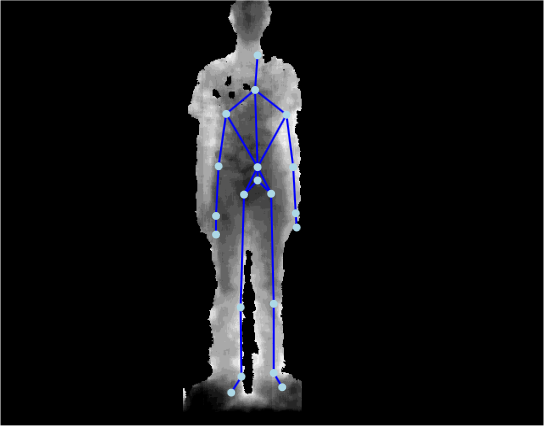
\includegraphics[scale=0.4]{images/parse3} 
\end{center}
\caption{Depth and hand based cut off, with colouring.}
\label{fig:depth and hand based cut off}
\end{figure} 
\section{Point Clouds}
\label{impl:point clouds}
\subsection{Data Structure}
The K-D tree data structure, discussed in section was partially implemented by a third party open source library, which was then generalised to accommodate the point structures. \\

Additional C\# primitive data structures were utilised to maintain meta information about the point cloud such as maximum and minimum values; information about the resolution of the image from the input device and data about the input device. \\ 

\subsection{Conversion to real world coordinates}
The conversion from a depth map to the real-world coordinate system is as follows. The depth map is scanned, progressively incrementing $i_x$ and $i_y$. At every stage the calculations in \ref{eq:pc conv x}, \ref{eq:pc conv y} and \ref{eq:pc conv z} are performed and then inserted into a \texttt{PointRGB} data structure along with the \emph{red}, \emph{green} and \emph{blue} values. An explanation of the variables in the equations just mentioned can be found in Table \ref{fig:pc conv meaning}. \\

\begin{equation}
    z = depthValue * scale
    \label{eq:pc conv z}
\end{equation} \\
\begin{equation}
    x = (centre_x - i_x) * z * f_{xinv}
    \label{eq:pc conv x}
\end{equation} \\
\begin{equation}
    y = (centre_y - i_y) * z * f_{yinv}
    \label{eq:pc conv y}
\end{equation} \\

\begin{table}[h!]
    \centering
    \begin{tabular}{ |c | c | c |}
    \hline
        Variable   & Meaning                  & Value \\ \hline
        $centre_x$ & centre of depth map (x)  & $\frac{640}{2}$ * \\
        $centre_y$ & centre of depth map (y)  & $\frac{480}{2}$ * \\
        $scale$    & fiddle factor            & $0.001$ \\
        $f_{xinv}$ & fiddle factor            & $\frac{1}{476}$ \\
        $f_{yinv}$ & fiddle factor            & $\frac{1}{476}$ \\  
        \hline
    \end{tabular}
    \caption[The meaning behind variables used in the depth map to point cloud algorithm]{The meaning behind variables used in the depth map to point cloud algorithm. * denotes a value that is specific to the PARSE implementation} 
    \label{fig:pc conv meaning}
\end{table} \\

\subsection{Merging point clouds}
There is no trivial way to attach on point cloud to another due to the way in which the K-D tree is structured. It is therefore necessary to take the points from one point cloud and then add them to the second one-by-one. Sometimes there are collisions, a point is defined in exactly the same place in the point cloud - especially in the overlapping areas after a good registration has taken place. When this happens the second point is simply discarded. \\

\subsection{Transformation}
To aid the registration process a number of key transformation functions have been implemented which operate directly on the data stored within the point cloud data structures. \\

\subsubsection{Translation}
The translation method simply works by translating all data in the point cloud and then translating the maximum and minimum values in each coordinate. \\

\subsubsection{Rotation}
The rotation method is slightly more complicated as rotation in a 3-D space necessitates the usage of the complex plane. The rotation is achieved through the utilisation of a quaternion and a rotation matrix. \\

\subsection{Floor removal}
A problem that occurred during the registration process was the floor getting in the way. This can be mitigated by calling the \texttt{removeFloor} method. The method simply removes the lower plane in the point cloud. \\

\subsection{Visualisation}
The visualisation was implemented using the Windows Presentation Framework with Helix 3D as a helper library. Each depth point in the point cloud was modelled as a small cube so that they may be displayed in a pleasing manner. Examples of visualisations may be seen throughout this report but specifically in section \ref{imp:stitching}.

%complete
\section{Point Cloud Stitching}
\label{design:registration}
\label{design:sitching} %legacy, do not remove
\label{design:stitching}
The specification states that only a single scanner is to be used. This necessitates the utilisation of multiple scans and the stitching thereof into one unified data structure. This data structure can then be manipulated to produce volume estimation, as described in Section \ref{design:volume estimation}. The process of stitching these point clouds together to create one unified dataset is known as \emph{registration}\cite{Makadia2006} which has been described in Section \ref{research:registration}. The development of ideas leading to the final algorithm will be described in this section.  \\

\subsection{Input Data}
Depth maps of people (shells) are to be passed to the registration algorithm from a \emph{person isolation} subsystem. 

\subsection{Design Pattern}
\label{design:design pattern}
The various point cloud stitching algorithms all extend a class called ``Stitcher``. This makes it easy for new stitching algorithms to be deployed within the PARSE environment as only a single line of code needs to be modified in order to use a different stitching algorithm.\\

\subsection{Initial Experimentation}
Initially the point clouds were stitched by rotating successive scans 90\degree \ , increasing by a further 90\degree \ for each previous scan that has been taken, in an anticlockwise direction. The scan was then translated by a constant vector to produce a reasonable point cloud. This was able to produce reasonable results in individual cases but people come in a variety of ``depths`` and such an algorithm would only be useful in a world where everyone had constant "depths". \\

\subsection{Development of a more sophisticated approach: Bounding Boxes} 
\label{design:bounding boxes}
\label{design:bounding box}
While the Kinect is designed to produce depth information, it is only capable of scanning the visible surfaces of objects in front of the point in the 3D world in which it is situated. This has led to the coining of the term \emph{2.5D} to explain the limited information that the Kinect, and all single depth sensors, are able to gain about the world around them \cite{lu2006}. In theory this very limitation can be exploited to produce a reasonable, but by no means perfect, point cloud registration most cases. Within the context of this project this has come to be known as the \emph{Bounding Box} method of point cloud registration. \\ 

\subsubsection{Scanning Phase}
As with the initial experimentation, the bounding box method requires four scans; $S_1, S_2, S_3, S_4$. After each scan is obtained the patient is rotated by 90\degree \ in an anti clockwise direction. Each scan contains length and width information which is used in the processing phase. These scans are then packaged into a list data structure and sent to the bounding box method for processing. \\

\subsubsection{Processing Phase}
The processing phase consists of a number of simple rotations and translations. The subject was only rotated about the vector $(0, 1, 0)$ which significantly reduced the complexity of the operations. Table \ref{tab:bb processing} shows the rotations and translations that were performed for each scan. \\

%table 
\begin{table}
    \begin{tabular}{| p{0.8cm}| p{1.4cm} | p{4.9cm} | p{3.9cm} |}
    \hline
        Scan & Rotation & Rotation Axis & Translation  \\
        \hline
        $S_1$ & 0 \degree & $(0, 0, 0)$ & (0,0,0)  \\
        $S_2$ & 90 \degree & $(S_2(x_{min}), S_2(y_{min}), S_2(z_{min}))$ & $(0, 0, width)$  \\
        $S_3$ & 180 \degree & $(S_3(x_{min}), S_3(y_{min}), S_3(z_{min}))$ & $(S_3(width), 0, S_2(width))$  \\
        $S_4$ & 270 \degree & $(S_4(x_{min}), S_4(y_{min}), S_4(z_{min}))$ & $(S_3(width), 0, 0)$  \\
        \hline
    \end{tabular}   
    \caption{The processing that takes place on each data item for the Bounding Box method}
    \label{tab:bb processing}
\end{table} \\

\subsubsection{Challenges}
Despite the apparent successful stitching in many cases, the \emph{Bounding Box} method produced erratic results occasionally. Due to anatomical differences, male subjects tended tended to be stitched more accurately than female ones. This was also the case with obese subjects. This problem has been internally known as the \emph{Breast Problem} (Section \ref{testing:the breast problem}). \\

To address this; a more sophisticated registration method, the Iterative Cloud Positioning (ICP) algorithm (Discussed in Section \ref{res:icp}) was investigated. One of the big problems with the ICP algorithm, and other registration algorithms, is that they require some form of initial alignment which is then improved over time. This initial problem had already been potentially solved using the Bounding Box method and so it has been utilised part of a processing pipeline. \\

\subsection{Manual Alignment}
As discussed in the previous section, it is necessary that some form of initial alignment is made before most algorithms would be useful. To address the breast problem (Section \ref{testing:the breast problem}) it could be possible to offer some kind of manual alignment of the body panels. This, however, would potentially introduce unpredictable human error and would require real-time visualisation and modification of the point cloud data structures. Performing just four rotations and one rendering, as in the Bounding Box method \ref{design:bounding box}, takes several seconds to complete and therefore a new trade-off of image resolution vs display and processing hardware would be introduced. The manual alignment idea was ultimately abandoned due to the overriding objective of keeping the final product cheap in terms of hardware requirements, accurate and easy for the operator to use. \\

\begin{figure}[h!!]
    \label{fig:registration pipeline}
    \begin{center}
        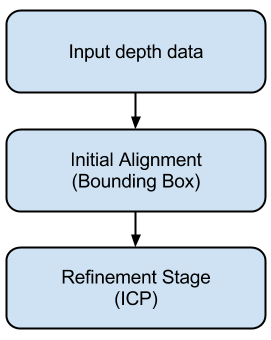
\includegraphics[scale=0.6]{zscreenshots/reg-pipeline.png}
        \caption{A pipelined approach towards registration}
    \end{center}
\end{figure}

\subsection{Final design: Iterative Closest Point (ICP) algorithm}
So far it has been explained how a simple method that is the bounding box method is able to produce reasonably good results. In Section \ref{res:icp} we learnt that the gold standard for registration is the Iterative Closest Point method which requires some initial alignment. This alignment could be provided by the bounding box method. \\ 

Using the information that from experimentation and the research in Section \ref{res:icp} a pipelined approach to registration was developed using the three steps, explained in Figure \ref{fig:registration pipeline}.


\section{Volume Estimation}
This section details the implementation of the chosen, SSP based volume estimation algorithm discussed in Section \ref{design:planimetry}. During this phase, several issues were overcome. \\

\subsection{How Many Planes?}
There was a necessary trade off between number of planes and quality of those planes. If the number of planes was too low, the volume estimation would be woefully inaccurate due to a lack of required granularity. If the number of planes was too high, then the volume would be inaccurate due to the lack of information contained within a plane. Sixty planes were chosen, based on a visual inspection of planes within the Corbett data set, shown in Figure \ref{fig:the_corbett_data_set}.\\

\begin{figure}[htb]
\begin{center}
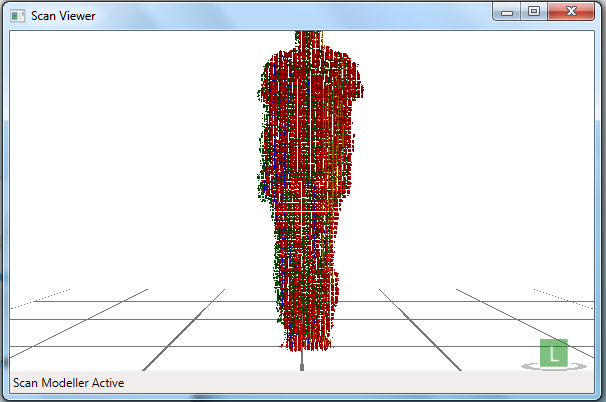
\includegraphics[scale=0.4]{images/corbett_dataset} 
\end{center}
\caption{The Corbett data set, stitched perfectly by the Bounding Box method}
\label{fig:the_corbett_data_set}
\end{figure}

\subsection{Noisy Data}
The data retrieved from the point clouds was not as originally expected. Firstly, the y-values were not discrete but continuous, as a result retrieving a plane at a single height would not result in ring of points. Therefore, a plane would be retrieved from a range of heights and then the points flattened to form a ring.\\

Also, the points were not close to a convex hull as expected, see Figure \ref{slice 30 from the corbett data set}, but were in fact quite noisy. As such, the points were \emph{sub-sampled} and then averaged to reduce noise. Sub-sampling by a factor of $n$ involved discarding $n-1$ points out of every $n$. Averaging points by a factor of $n$ involved adding the co-ordinate values of $n$ points, averaging them into a single point and returning a list of such average points. Figure \ref{plane 30 from the corbett data set sub-sampled and averaged} shows plane 30 of the Corbett data set after being sub-sampled and averaged by a factor of 7. A factor of 7 was chosen again based on visual inspection of the planes.\\

\begin{figure}[htb]
\begin{center}
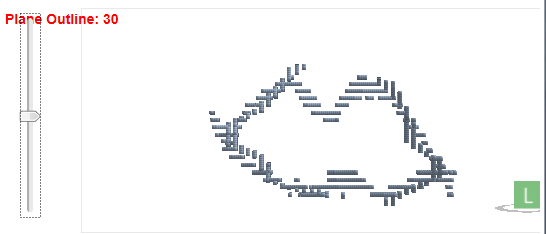
\includegraphics[scale=0.4]{images/notasexpected} 
\end{center}
\caption{Plane 30 from the Corbett data set}
\label{slice 30 from the corbett data set}
\end{figure} \\

\begin{figure}[htb]
\begin{center}
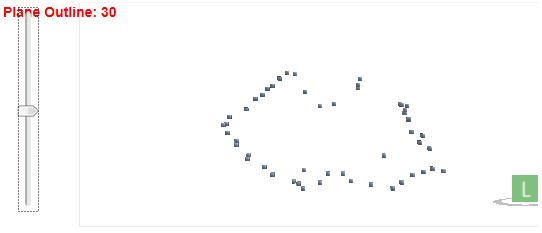
\includegraphics[scale=0.4]{images/improved} 
\end{center}
\caption{Plane 30 from the Corbett data set sub-sampled and averaged}
\label{plane 30 from the corbett data set sub-sampled and averaged}
\end{figure} \\

\subsection{The Need for a Transform Constant}
Early metrics returned were calculated in \emph{point cloud space} (PCS), as evidenced by the Corbett data subject's height being predicted as 2.27m. Therefore, a transform constant is required to move between measurements calculated in point cloud space (PCS) and measurements in terms of SI units in \emph{real world space} (RWS). Such a transform was believed necessary because the Kinect stores distances in terms of pixels and points, rather than meters and it is real world measurements that the calculated volume should be given. The transform was suspected to be multiplicative and as such is of the form shown in equation \ref{imp: transform between pcs and rws}. Determination of this constant was determined empirically during testing.\\

\begin{equation}
Volume_{PCS} * Transform Constant = Volume_{RWS}
\label{imp: transform between pcs and rws}
\end{equation}\\
\section{Limb Circumference}
\label{design:limbcircum}

The design of algorithms used for calculating limb circumference builds on the design principles of planimetry and as identified in section 3.6.1, this forms a reasonable basis for calculating circumferences using range imaging. 

\subsection{Plane Partitioning}

The limb circumference approach uses the sames SSP methodology for the estimation of volumes, pulling out planes using the shoelace formula. Hence limb circumference will operate on the same basis of the full body scan. Due consideration was given to alternative scanning contexts, where localised scanning would take place around a particular limb. However, as per the functional requirements of the system, we wanted to minimise the amount of configuration and patient setup required for the capturing of these measurements. The resolution of the Kinect device for capturing and tracking limb circumference, with it's 11-bit depth and 2048 levels of sensitivity was deemed adequate for estimating these metrics at distance. \\

Plane partitioning is achieved by using a mapping between the skeletal feature points and the point cloud isolated from the depth map. The 20 skeletal feature points are defined in terms of \emph{real-world coordinates} inferred from the depth map representation. The $(x,y,z)$ co-ordinates of these feature points are related by the inferred body part identification. With this, a bounding box around the limb is first determined in real-world coordinates. These bounds are defined by taking the minimal and maximal x,y coordinate's from the feature points for the limb. These bounds are then transformed into the point cloud co-ordinate system. The relative depth of the limb skeletal feature points are identical to the depth of the point cloud and as such do not require this transformation. \\

\begin{figure}[ht]
\begin{center}
$PC_n_e_w(x,y) = ((C_x,C_y) - (x,y)) * zz * f_x_,_yinv$
\end{center}
\caption{Translation from Real-world to Point Cloud co-ordinate system}
\label{fig:conversionformula}
\end{figure}

$C_x$ and $C_y$ are defined as the centre of the captured depth map of resolution 640x480 pixels. The depth map is then scaled by a constant $zz$ defining the size of the points that will be used to represent the point cloud in the 3D visualisation. The point is then multiplied by the invariants $f_x_,_yinv$. The importance of using this arbitrary point cloud space is highlighted by the unique set of points it generates that can then be represented accurately. It also allows information defined in real-world coordinates such as a the aforementioned skeletal data to be associated with each captured point cloud.

\subsection{Circumference Calculation}

The algorithm then subsamples on the n returned planes from the partitioned point cloud but uses the planes equidistant between the limb joints to give a mean representation of limb circumference on the selected limb. The circumference of each plane is calculated using the \emph{Gift Wrapping} algorithm, as detailed in the research section of the report, which returns the convex hull of a set of points. In the case of the PARSE implementation, we pass a subsampled region of planes and for each y return a convex hull which is then averaged for the mid-region for the particular limb. Similar to the estimation of Volume, the circumference returned is not defined in terms of SI units but rather determined in terms of the point cloud. This will require further testing to ascertain a suitable multiplicative constant to obtain a reasonable approximation to the circumference of the subject. \\

\subsection{Algorithm Running Time}

This algorithm enumerates each limb and performs plane partitioning and circumference calculation in real time. Because the algorithm itself is derived from the volume calculation and planimetry used to calculate whole-body volume, it is sensible to assume a similar running complexity to $O(\sqrt[3]{p}^2)$. The running complexity of calculating limb circumference is further compounded by the limb enumeration and bounding box calculation step where $O(n)$ represents the possible number of times the planimetry algorithm is to be run and $O(n^2)$ for each bound for those limbs to be calculated.

\subsection{Alternative Approaches}

Apart from the direct partitioning of this abstract point cloud structure and the calculation of the convex hull for each of the extracted planes, there are other means of limb circumference measurement that uses least squares regression for the fitting of ellipses to scatted 3 dimensional data, something that could be easily extended to calculation of circumference for a given point cloud region based on the fitted ellipses. Fitzgibbon et al. \cite{Fitzgibbon1999} fit these primitive ellipses to provided image data by finding the set of parameters that minimise the distance between the provided data points and the proposed ellipse shape.  While this least squares method is only used on scattered data in 2 dimensional space, this method could be viably extended into 3D space as has been achieved by Geiger who proposes a method which registers the persons point cloud in different poses and projects the captured 3 dimensional data into 2D space for registering the circumference as the person rotates \cite{Geiger2011}.



\section{Markerless Recognition}
The markerless recognition problem was approached in two phases. First, the sensor's location was to be tracked using the video image feed from the Kinect. Then, this location would be translated into 3D space using information from the depth feed, and finally the sensor's position relative to the body could be calculated. This mechanism could then be used either just once, to register a new position, or on every frame, to guide the sensor to a target position.\\

Three different algorithms were tested for effectiveness in the application: one robust algorithm - SURF, a non-robust algorithm - Haar classification, and a simple colour search.\\

\subsection{Colour Search}
The colour search tests intend to answer three questions:
\begin{enumerate}
\item How effective is searching for a specific colour?
\item How much difference is there between searching the RGB and HSL colour spaces?
\item What is a ‘good’ colour to search for?
\end{enumerate}

In order to answer these questions, the colour searching mechanism must allow for ranges of colours to be searched for, and in either of the RGB or HSL colour spaces. \\

For testing, a separate application was designed, which would analyse the video feed from the Kinect. A simple check highlighted values in the output image on a binary basis: matches in white, the rest in black. A more efficient algorithm, if needed, would be put in place during any further development.\\

\subsection{Haar}
Early in the project, Haar classifiers were considered to be a viable option. Highly rated by users of the imaging library PCL, in use by the project at that time, the Haar classifier appeared worthy of testing. The premise was that, once trained on sufficient data, a Haar classifier could be applied to imagery in real time, thus giving a highly responsive tracking system.\\

The PCL imaging library provides numerous algorithms written in C, available within a C# wrapper. This gives the user the potential to create a highly efficient program. Such usage does however expose the library’s C heritage with the requirement in many places to pass in memory allocations and pointers, which is a drawback for some. \\

The initial design plan was to first learn the classifier generation procedure, and then run basic tests on its effectiveness. If sufficiently reliable, a system would then be devised which could use a collection of classifiers in parallel. One of the drawbacks of Haar classifiers is their sensitivity to rotational variance. This is acceptable in many situations, for example face detection in photographs, but would not be helpful in the defined situation of this project. Thus, a system would be devised and tested, which would utilise a collection of classifiers generated for the target at different rotations.\\

\subsection{SURF}
The OpenCV library provides an implementation of the SURF algorithm, and this was used to create a classifier suitable for testing. This, combined with SURF's reputation for high speed, led to it's use over SIFT. In reality, however, it was not possible to run this SURF implementation in real time. Each SURF run took a few seconds, which made video or real-time testing impossible. The SURF classifier was therefore tested only on static images. \\

The default parameters were investigated, and the setup was deemed sufficient for the tests.\\

The program was configured to output a single image containing, on the right side, the target image with its features highlighted, and on the left side the input image with its features highlighted. Any correspondences between the two images’ features are indicated with lines, and any target identified is indicated by a rectangle.\\

\subsection{Scan Process}
The method for taking a tracked scan needed to be as simple as possible, and make intuitive actions where possible. One such measure is to allow automatic triggering of the capture event when the scanner is held still. This should mean that, once started, no further interaction with the computer is necessary to complete the scan process - an important time-saving feature, should the operator be working alone.\\

Once initiated, the scan process will immediately begin searching for and tracking the target sensing device, the operator and the patient. After determining the operator and the patient, the program will wait for the sensing device to be held still for a number of seconds before automatically triggering the capture routine, and closing the window.\\


\newpage
\section{Summary}
This section summaries the implementation phase of the project.\\

\subsubsection{Person Isolation}
The depth and colour based isolation, described in Section \ref{design:person isolation}, was implemented with out change to the design. However, colour based isolation was insufficient to create a point cloud and did not map well into depth space. Hence, the depth based isolation was chosen to proceed with.\\

\subsubsection{Registration}
From the data provided by the \emph{person isolation} algorithm the registration algorithm, described in Section \ref{design:registration}, produced good results that were usable in subsequent algorithms. The results from this algorithm were then saved and utilised by the \emph{volume estimation} and \emph{limb circumference} subsystems. 

\subsubsection{Volume Estimation}
The volume estimation has been implemented as designed with sub-sampling and averaging to reduce noise. From the planes pulled out for volume estimation also had their circumference measured, to do this, the sub-sampled and averaged plane was then turned into a convex hull.\\ 
 
\subsubsection{Markerless Recognition}
Test rigs were implemented to assess the effectiveness of the chosen algorithms. As testing later showed that robust algorithms perform poorly in this application, the RGB colour space search was chosen as the basis for the end product. Problems such as coordinate space conversion and subject \& operator identification were solved.